\chapter{Design}

I dette kapitel beskrives design-delen af hardware og software for SRM. På baggrund af arkitekturen redegøres der, hvordan HW/SW-blokkene, som indgår i arkitekturen er designet samt deres funktion. Designet for HW-delen indeholder diagrammer samt beregninger af komponentværdier. Desuden indeholder HW-delen en kort
beskrivelse af designovervejelser i forhold til de enkelte hardwareenheder. SW-designet beskriver funktioner og GUI samt særligt interessante dele af den interne logik i funktioner. 


\section{Hardware}

Dette afsnit omhandler designet af hardwaren, som anvendes til at måle  bioimpedans- og EMG-siganler. Figur \ref{fig:Blokaede} viser de komponenter, som skal anvendes for at SRM kan blive realiseret. SRM består af både designet komponenter og kommercielle komponenter. Disse kommercielle komponenter omfatter en Analog Discovery, en pc, en EMG-måler og er ikke blevet designet. Der er i stedet for set på om de kan leve op til de krav, som er nødvendige for at realisere det ønskede produkt. 


\begin{figure}[H]
\centering
{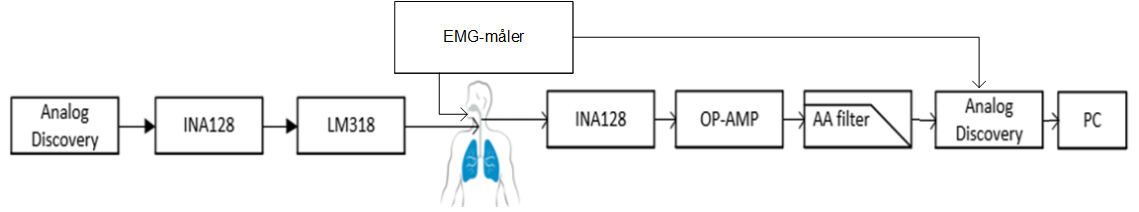
\includegraphics[width=\textwidth]
{Figure/Blokaede}}
\caption{Figuren viser de enkelte komponenter, som skal designes for at realisere SRM.}
\label{fig:Blokaede}
\end{figure}

\subsubsection{Analog Discovery}

AD har i dette bachelorprojekt to formål, at fungerer som funktionsgenerator og som dataopsamlingsmodul. Figur \ref{fig:ADogINA128} viser disse to formål. Det ene formål er at funktionsgeneratoren laver et AC signal med ampiltuden på 2 V og 20 kHz, som sendes til indgangen af instrumentationsforstærkeren INA128. Signalet bliver brugt til at generere en konstant strøm ud af operationsforstærkeren LM318N. Det andet formål er at AD modtager signal fra anti-aliaseringsfilter, som bliver konverteret fra analogt til digitalt signal.

\begin{figure}[H]
\centering
{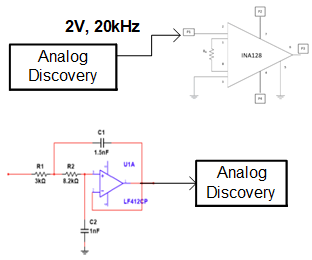
\includegraphics[width=10cm]
{Figure/ADogINA128}}
\caption{Figuren viser AD's funktion i det samlede system. AD fungerer som funktionsgenerator og som dataopsamlingsmodul.}
\label{fig:ADogINA128}
\end{figure}

Generelt for at foretage korrekt dataopsamling af signalet fra analogt domæne til digitalt domæne, skal Shannons samplingsteori overholdes. Det vil sige at samplingsfrekvensen skal minimum være det dobbelte af den maksimale frekvenskomponent, Nyquist-frekvensen. Frekvenser større end Nyquist-frekvensen giver anledning til aliasering. Dette vil resultere i et fejlsignal. Derfor vælges der en samlingsfrekvens som er væsentlig højere end den maksimale frekvenskomponent. 

Valg af dataopsamlingsenhed har også betydning for overgangen fra analogt domæne til digitalt domæne. Her konverteres de analoge værdier til de nærmeste digitale værdier. Konverteringen bestemmes af ADC'ens spændingsområde og opløsning. Forholdet i mellem spændningsområde og opløsning, udtrykkes LSB. LSB er et udtryk for den mindste detekterbare spændningsændring som ADC'en kan detektere. I henhold til AD's datablad, se \nameref{bilag15}, er denne opløsning på 14 bit, samtidig med et spændningsområde på 8 V, resulteret i en mindste spændningsændring som AD kan detektere 0,48 mV. Der henvises til \nameref{bilag5}, for den fulde udregning af LSB.

Derfor er det besluttet at bruge AD, da den har følgende fordele:
\begin{itemize}
\item Den kan fungere som funktionsgenerator samtidig med, at den læser to signaler ind simultant
\item Den kan sample to signaler simultant med en samplingsfrekvens på 500 kHz
\item Den kan fungere som dataopsamlingsenhed
\end{itemize}



\subsubsection{Instrumentationsforstærker}

Instrumentationsforstærkeren i dette bachelorprojekt, har til formål at undertrykke støj fra måleobjekt og efterfølgende forstærke signalet, men også forstærke indgangssignalet fra AD's funktionsgenerator. Derfor anvendes i dette
projekt to instrumentationsforstærker af typen INA128P. INA128P specifikationer kan læses i \nameref{bilag15}. INA128P giver mulighed for at forstærke signalet vha. kun en modstand. Fordelene ved anvendelse af instrumentationsforstærker, når det ønskes at måle elektrofysiologiske signaler er\cite{PeterJohansen2014}:
\begin{itemize}
\item 	Høj indgangsimpedans på ca. $10^{10} \Omega $
\item	Stor common mode rejection (CMR) på minimum 120dB
\item 	Differentielt input-single ended out (nødvendigt for at mindske $CM_{noise}$)
\end{itemize}



\textbf{Instrumentationsforstærker 1}

Den ene INA128 benyttes til at forstærke signalet og undertrykke støj fra AD's funktionsgenerator. Det ønskes at forstærke de 2 V fra AD til 4 V. Det vil sige at gain er 2 og derfor kan R$_{G}$ modstanden beregnes til 50 k$\Omega$. Udregning af R$_{G}$, diagram og stykliste kan ses i \nameref{bilag5}.





\section{SW}

Desuden indeholder bilaget et sekvens
diagram, der giver en detaljeret beskrivelse af udvalgte funktioner/metoder, som styrer
SRM hardware del.